\definecolor{LightGreen}{RGB}{102,194,165}
\providecommand{\iRef}[1]{{\tiny\color{HallowGreen} $[$#1$]$}}

\author[Tanjona Rabemananjara]{}
\institute{University of Milan}

\subsection{PDF replica compression}

\begin{frame}{Compression \& GAN Methodologies}
	\begin{columns}[T] 
		\begin{column}{.5\textwidth}
			\underline{Error Function (ERF):}
			\begin{equation*}
				\mathrm{ERF}_k = \frac{1}{N_k} \sum_{i}
				\left( \frac{C^{k}(x_{i}) - P^{k}(x_{i})}{P^{k}(x_{i})} \right)^2 
			\end{equation*}
			\begin{equation*}
				\mathrm{ERF}_\text{ToT} = \frac{1}{N_{\text{EST}}} \sum_{k} \mathrm{ERF}_k
			\end{equation*}
		\begin{itemize}
			\item $P^{k}$ is the value of the estimator $k$ for the \textcolor{blue}{PRIOR}
			\item $C^{k}$ is the value of the estimator $k$ for the \textcolor{magenta}{COMPRESSED}
			(either drawn from the \textcolor{blue}{PRIOR} or \textcolor{red}{ENHANCED} set)
		\end{itemize}
		\end{column}
		\hfill
		\begin{column}{.5\textwidth}	
			\underline{GANPDFs flowchart}:
			\begin{center}
				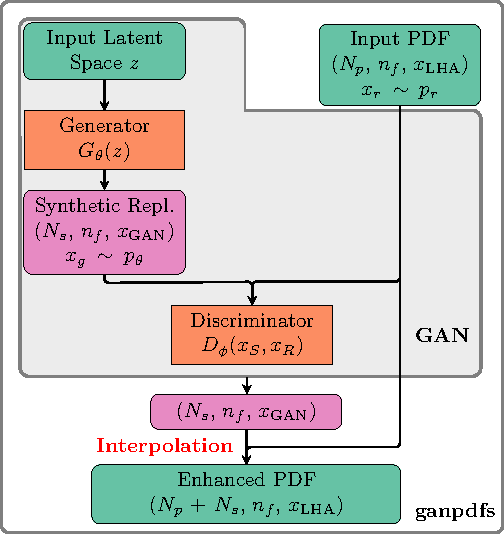
\includegraphics[height=.7\textheight]{./gan_compressor/imgs/gan-standalone.pdf}
			\end{center}
		\end{column}
	\end{columns}
\end{frame}

\begin{frame}{Final compressed sets}
	\underline{Number of Synthetic replicas in the compressed set}:
	\begin{columns}[T] 
		\begin{column}{.5\textwidth}
			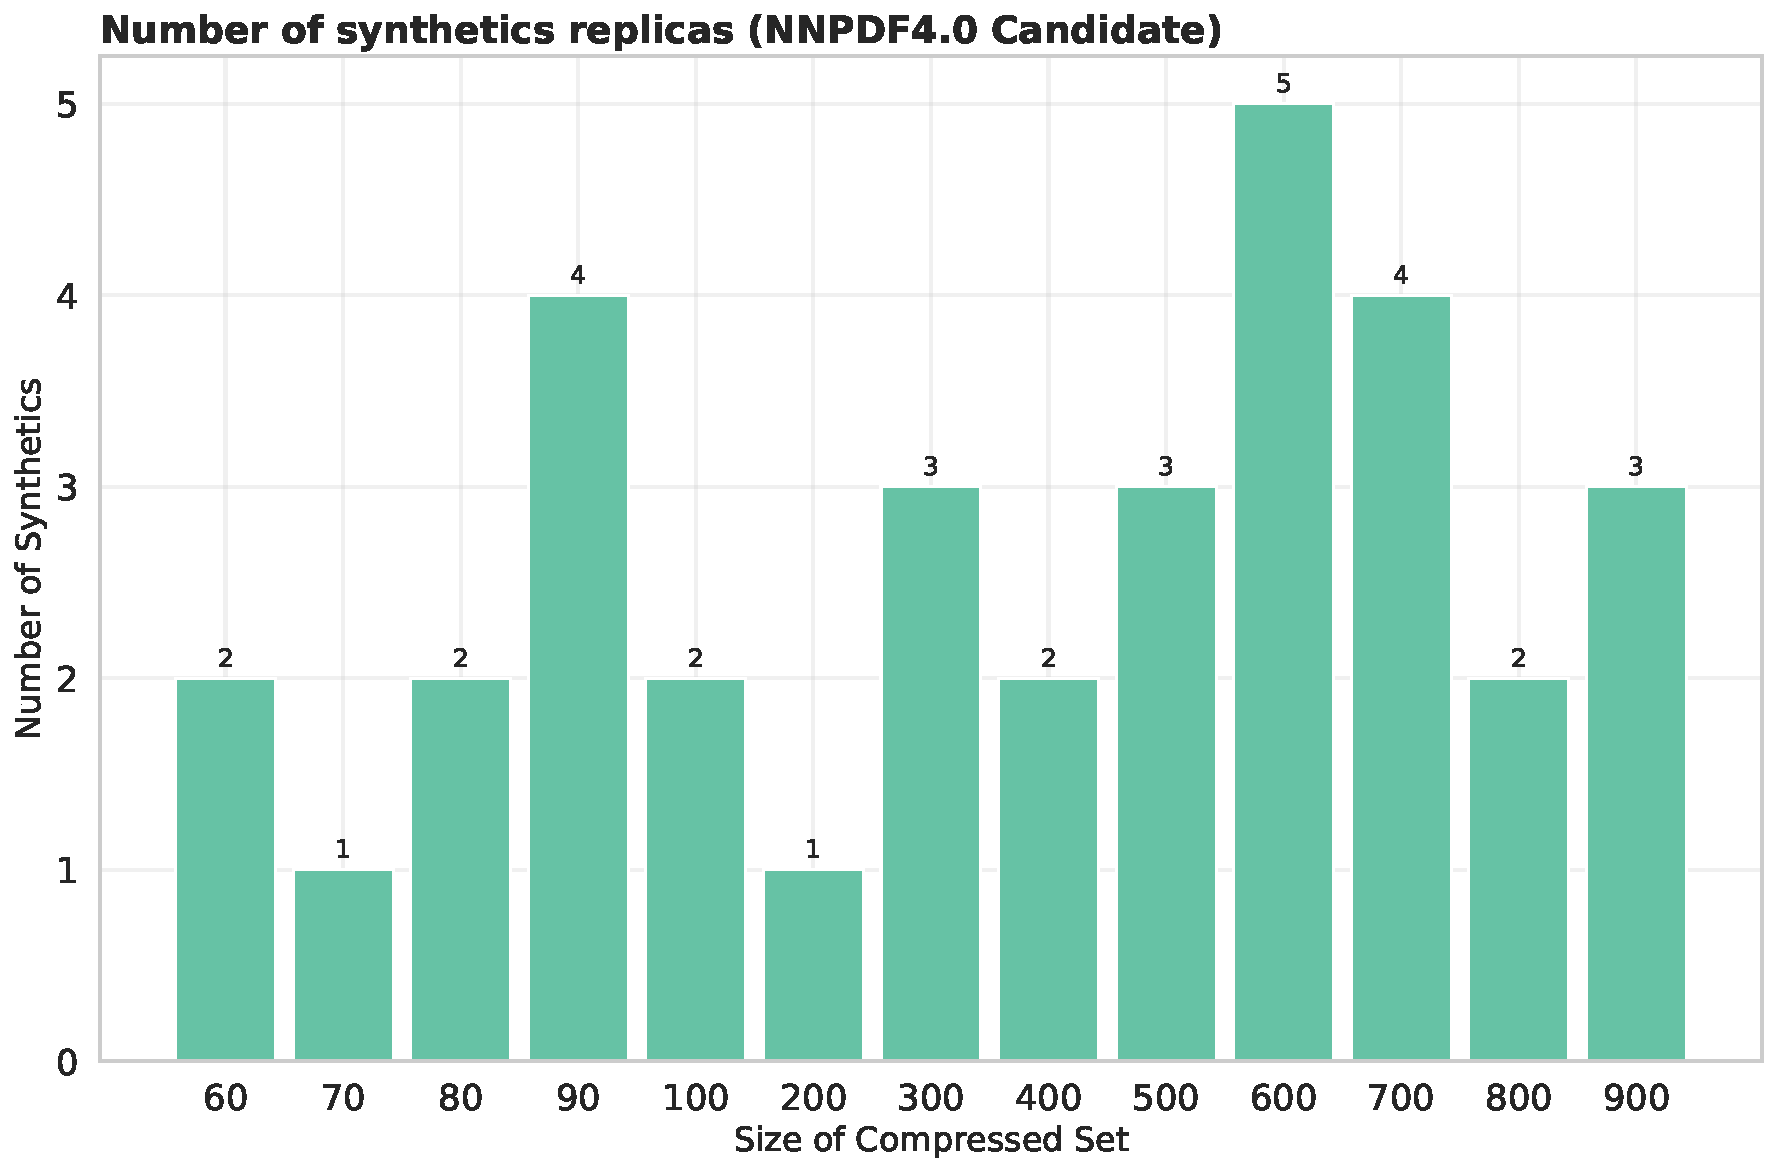
\includegraphics[width=\linewidth]{./gan_compressor/imgs/countings-nnpdf41.pdf}
		\end{column}
		\hfill
		\begin{column}{.5\textwidth}	
			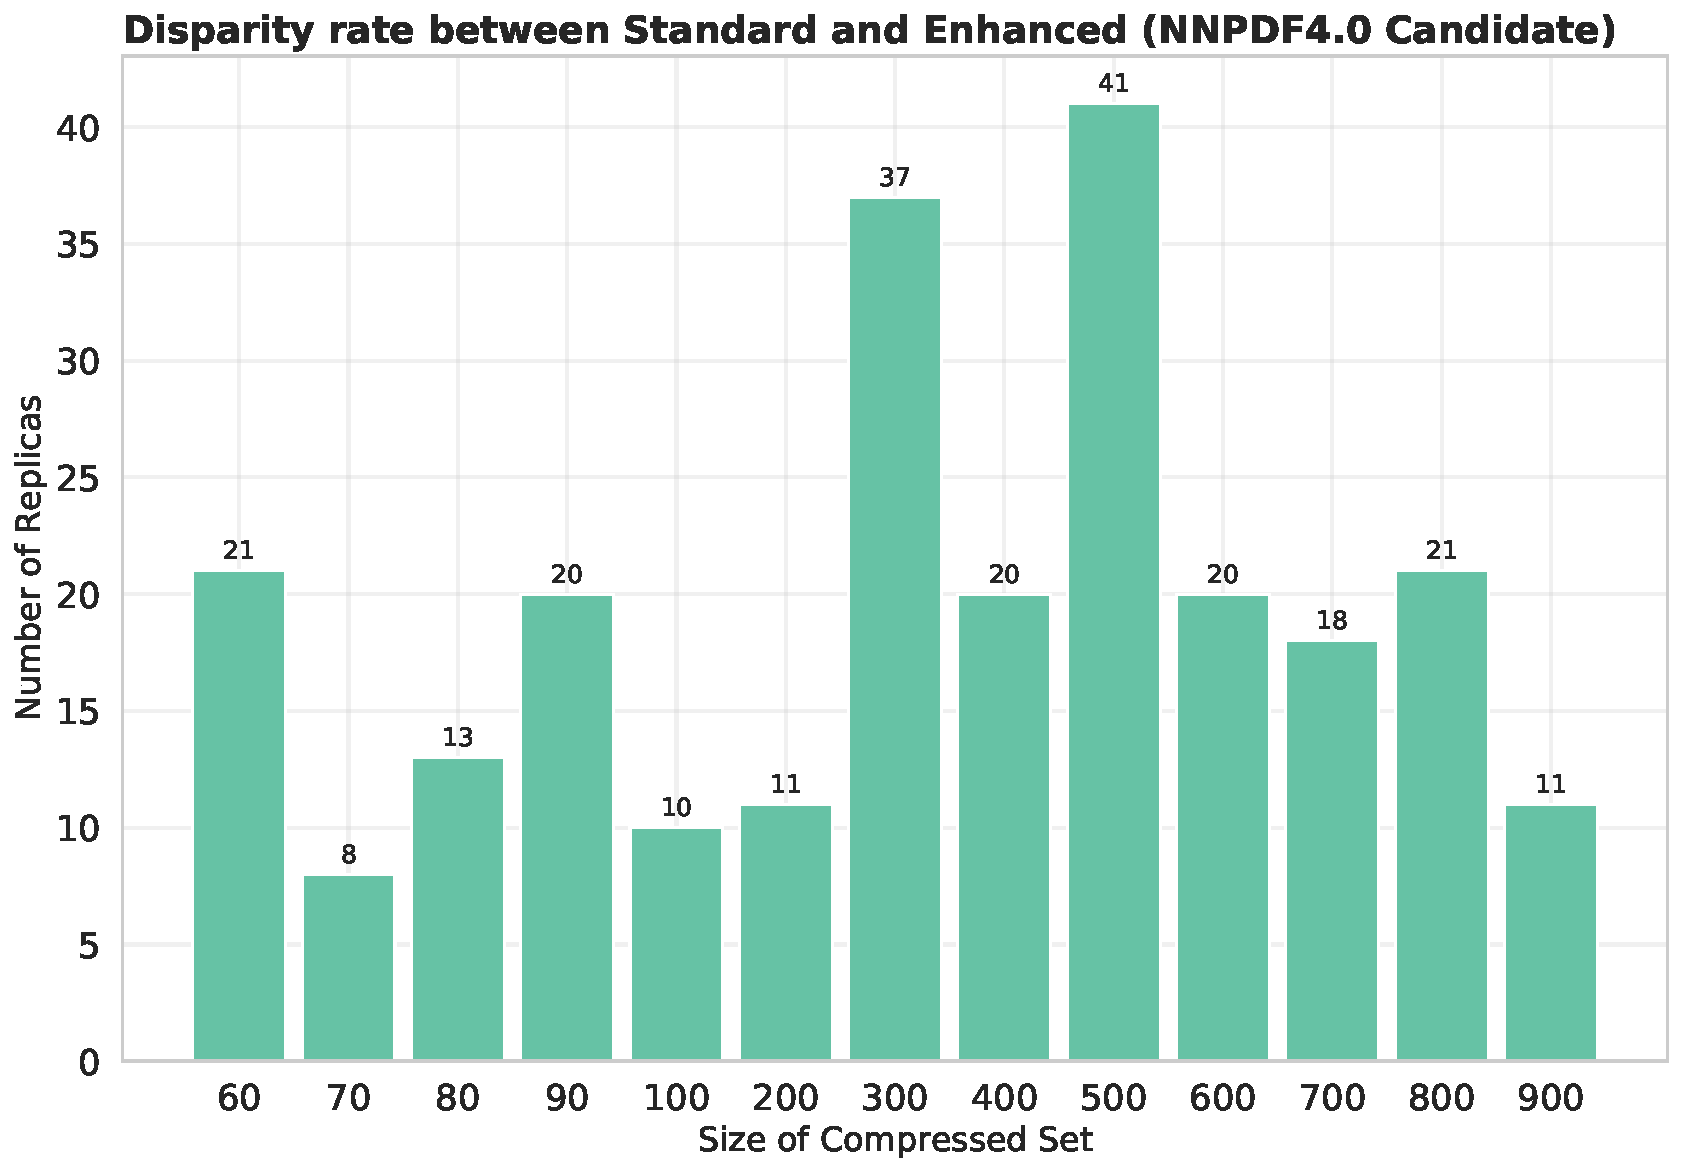
\includegraphics[width=\linewidth]{./gan_compressor/imgs/disparity.pdf}
		\end{column}
	\end{columns}
\end{frame}


\begin{frame}{Comparing PDF correlation matrix}
	\begin{columns}[T] 
		\begin{column}{.5\textwidth}
			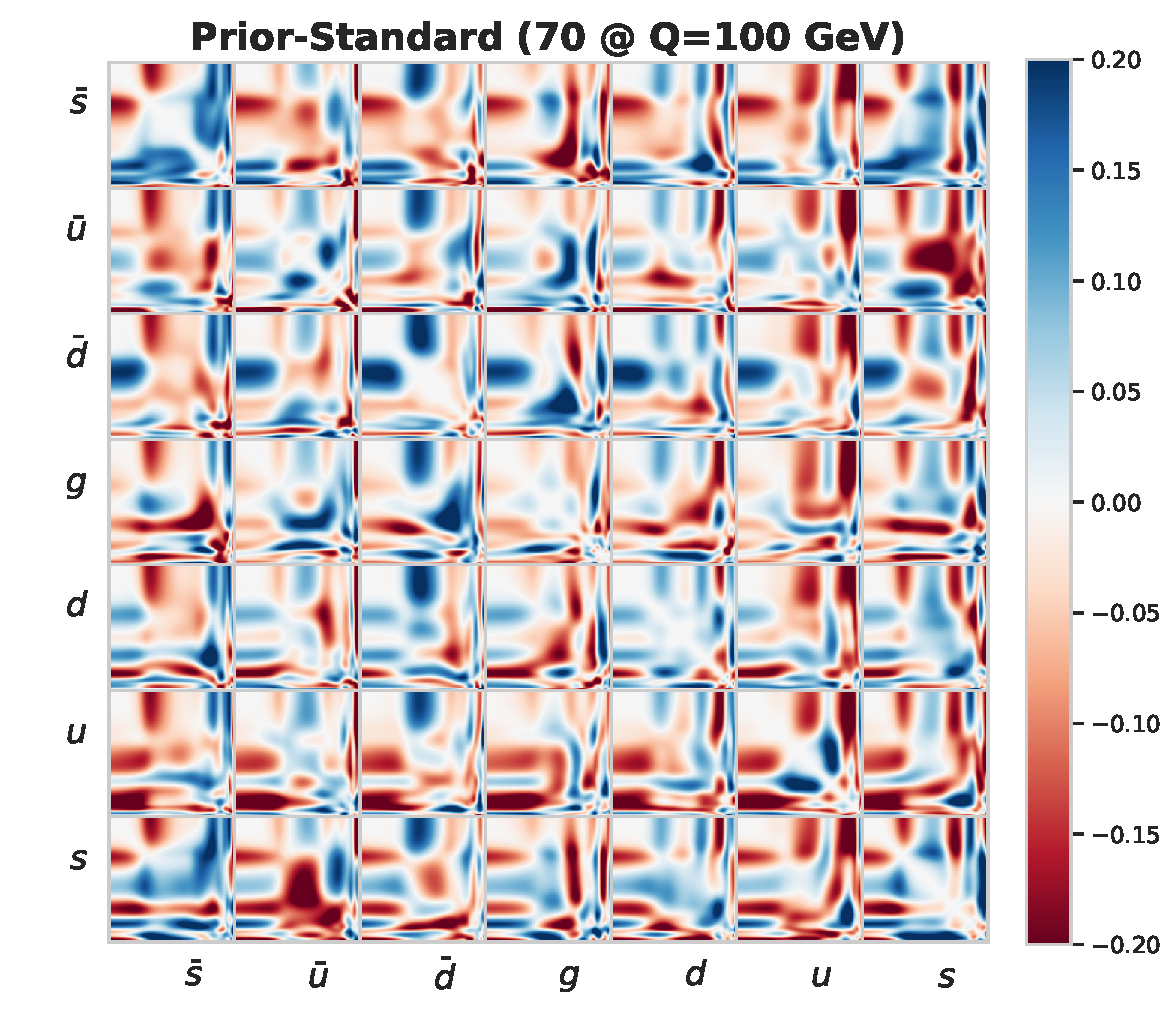
\includegraphics[width=\linewidth]{./gan_compressor/imgs/P_vs_S-N70.pdf}
		\end{column}
		\hfill
		\begin{column}{.5\textwidth}	
			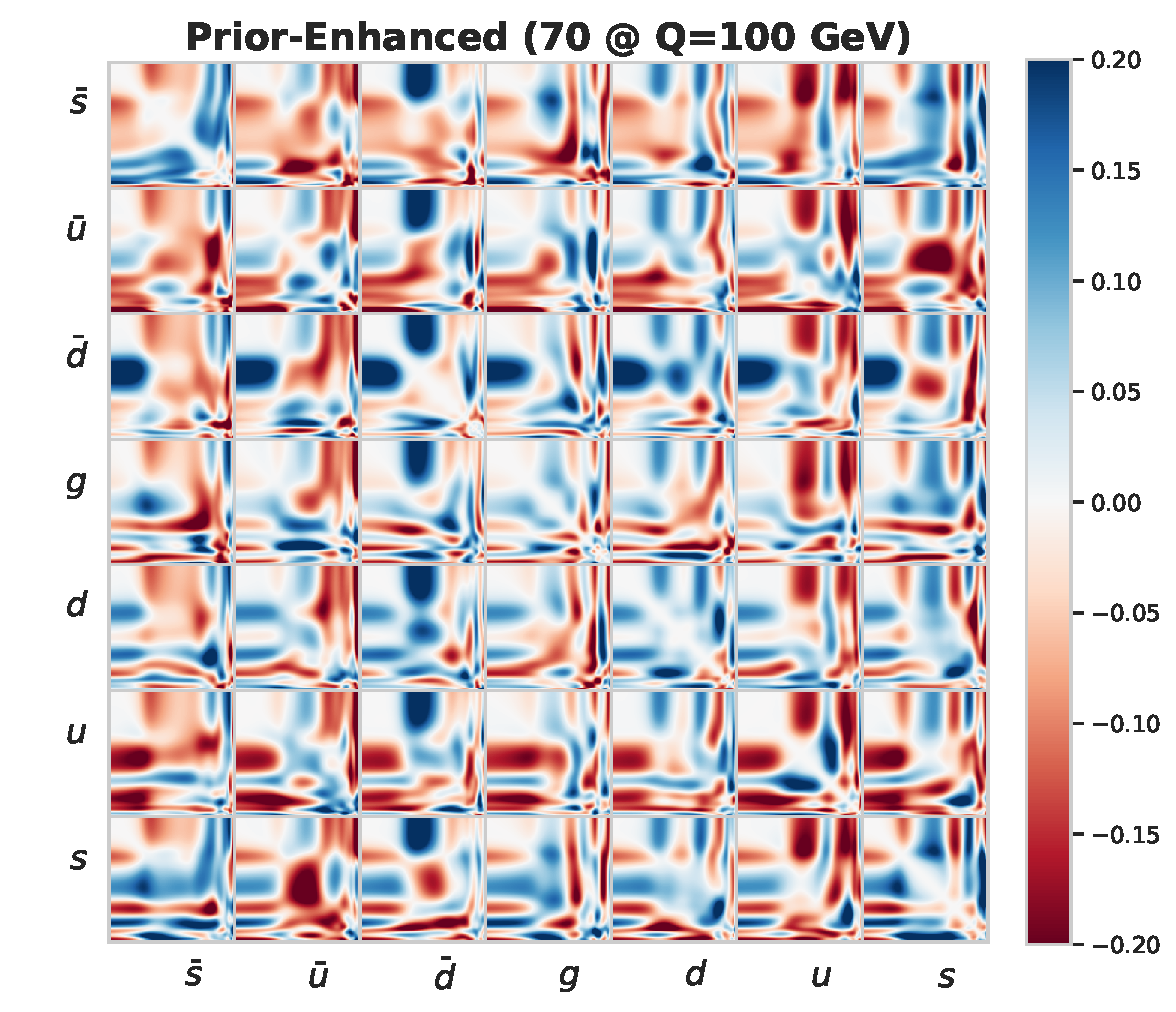
\includegraphics[width=\linewidth]{./gan_compressor/imgs/P_vs_E-N70.pdf}
		\end{column}
	\end{columns}
\end{frame}


\begin{frame}{Positivity Constraints}
	\begin{columns}[T] 
		\begin{column}{.5\textwidth}
			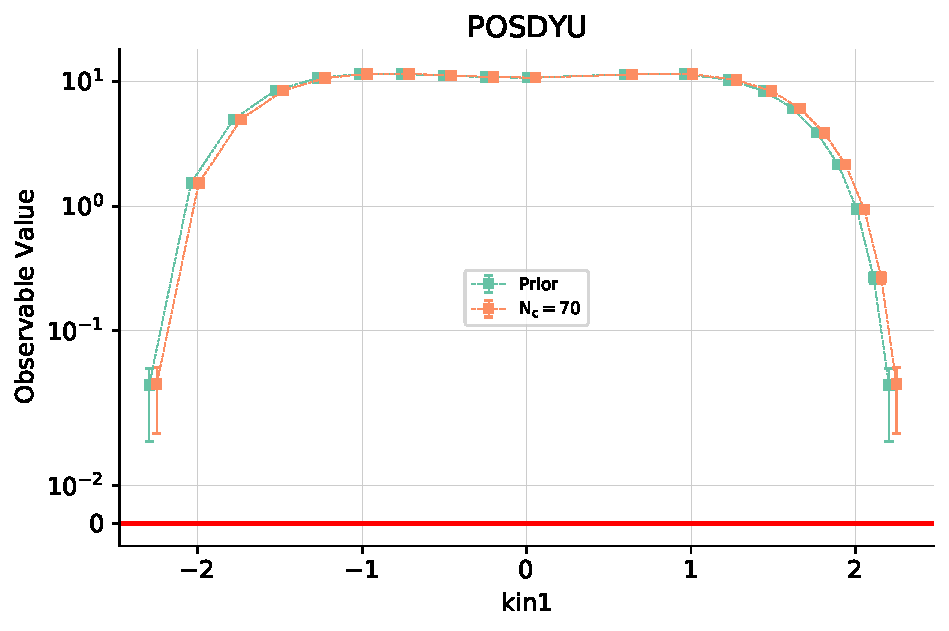
\includegraphics[width=\linewidth]{./gan_compressor/imgs/POSDYU.pdf}
		\end{column}
		\hfill
		\begin{column}{.5\textwidth}	
			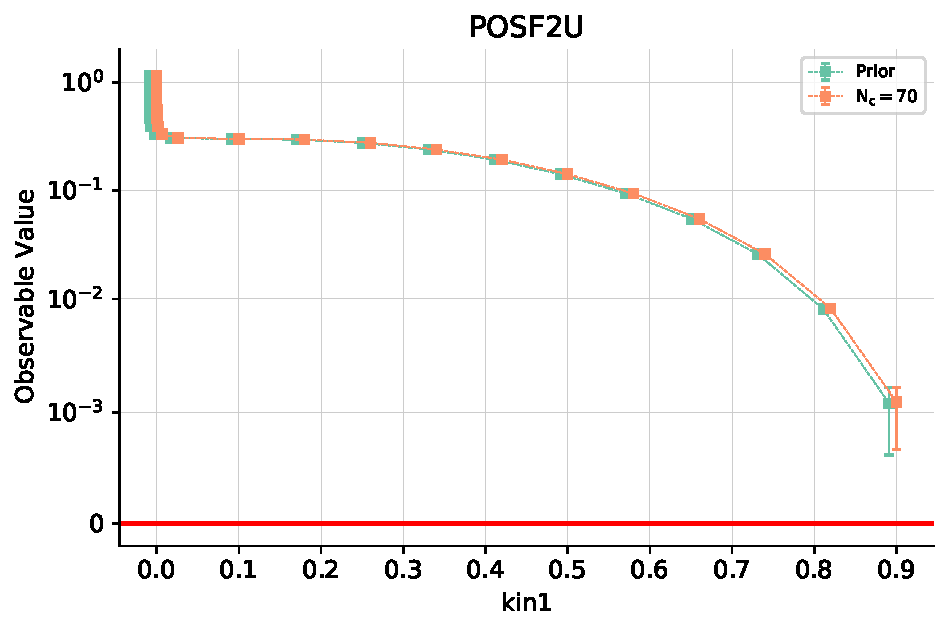
\includegraphics[width=\linewidth]{./gan_compressor/imgs/POSF2U.pdf}
		\end{column}
	\end{columns}
\end{frame}


\begin{frame}{GANs for PDF fitting}
	Consider 3 different set of fits:
	\begin{itemize}
		\item 2 disjoint fits $S_1$ and $S_2$ with $N=500$ replicas
		\item GAN fit $S_3$ with with $N=500$ replicas determined from $N_0=100$
	\end{itemize}
	\textcolor{LightGreen}{\textbf{GREEN}$\equiv \text{ERF}(S_1,S_2)$} and \textcolor{orange}{\textbf{ORANGE}
		$\equiv \text{ERF}(S_1,S_2)$} using different resampling methodologies.
	\begin{columns}[T] 
		\begin{column}{.5\textwidth}
			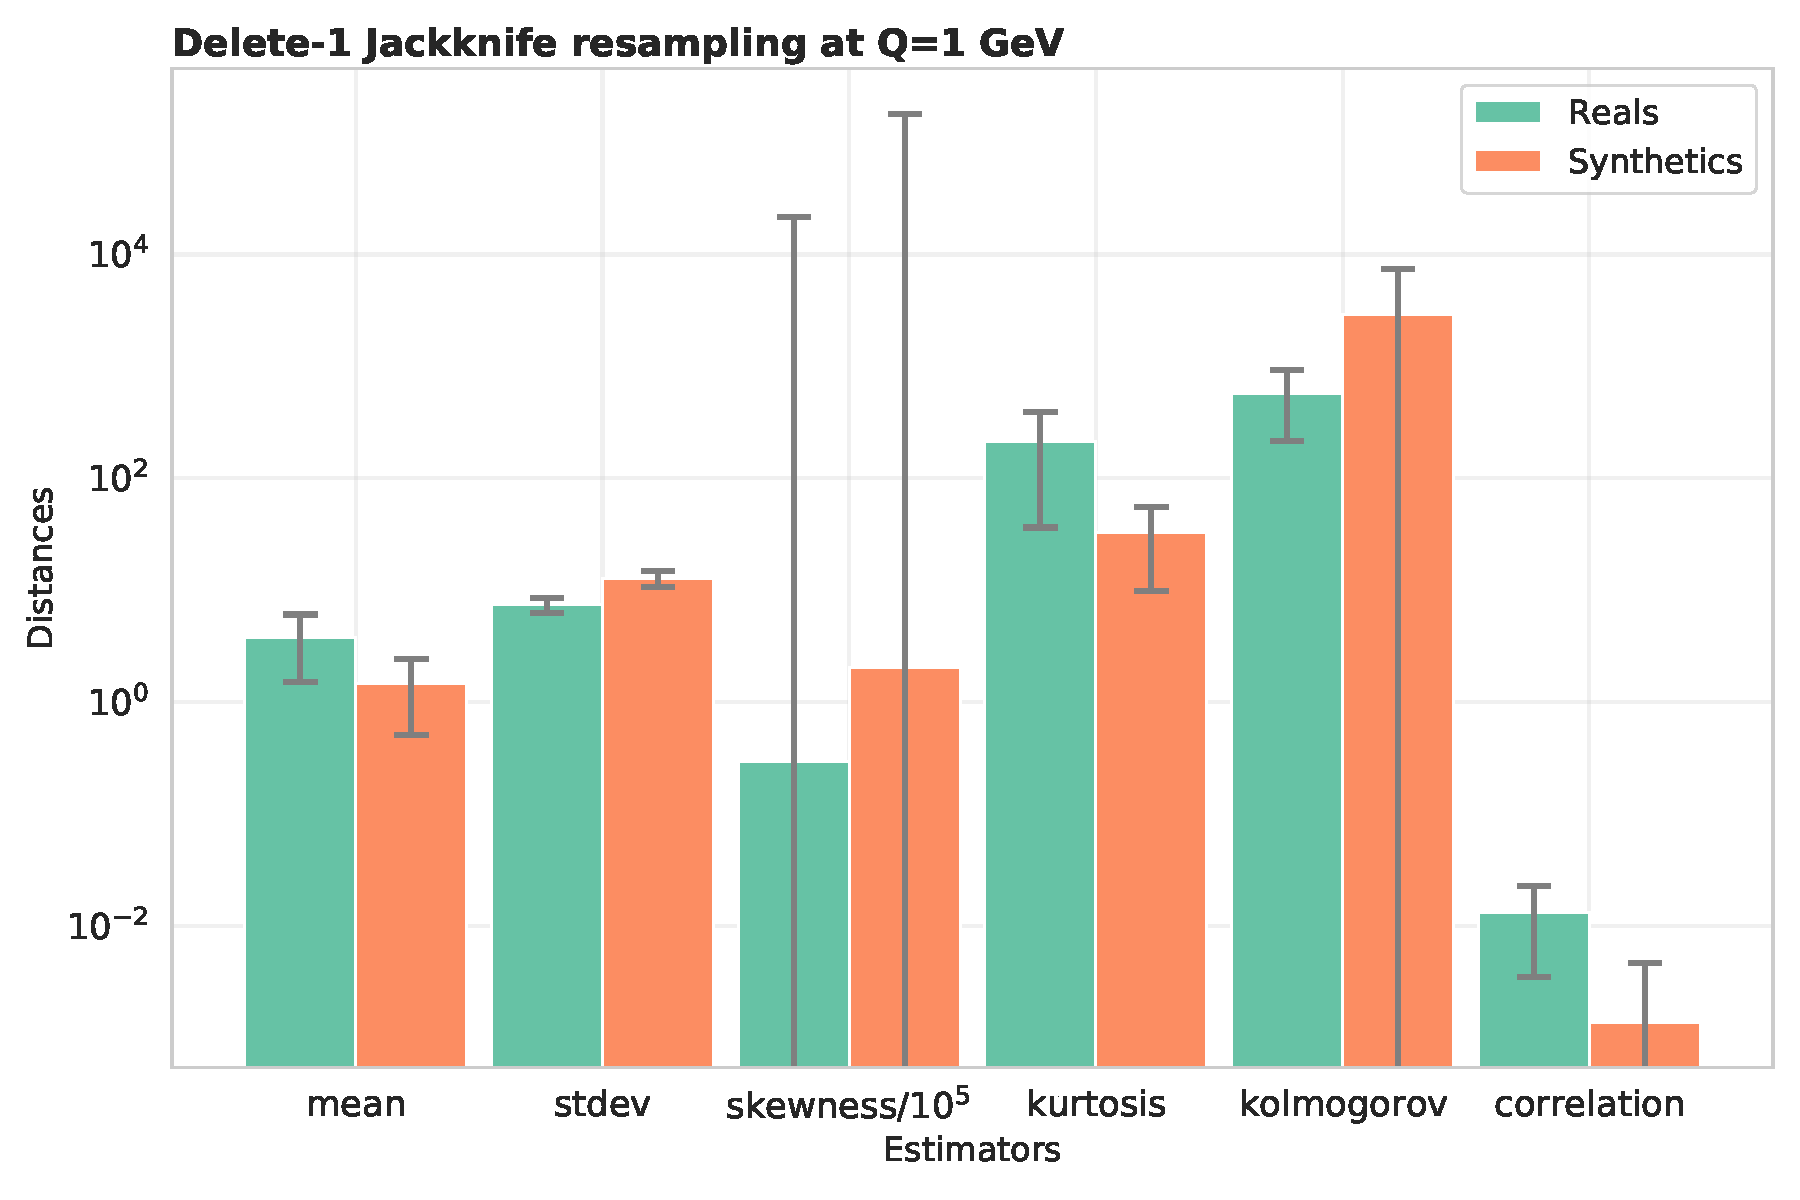
\includegraphics[width=\linewidth]{./gan_compressor/imgs/jackknife-v1.pdf}
		\end{column}
		\hfill
		\begin{column}{.5\textwidth}	
			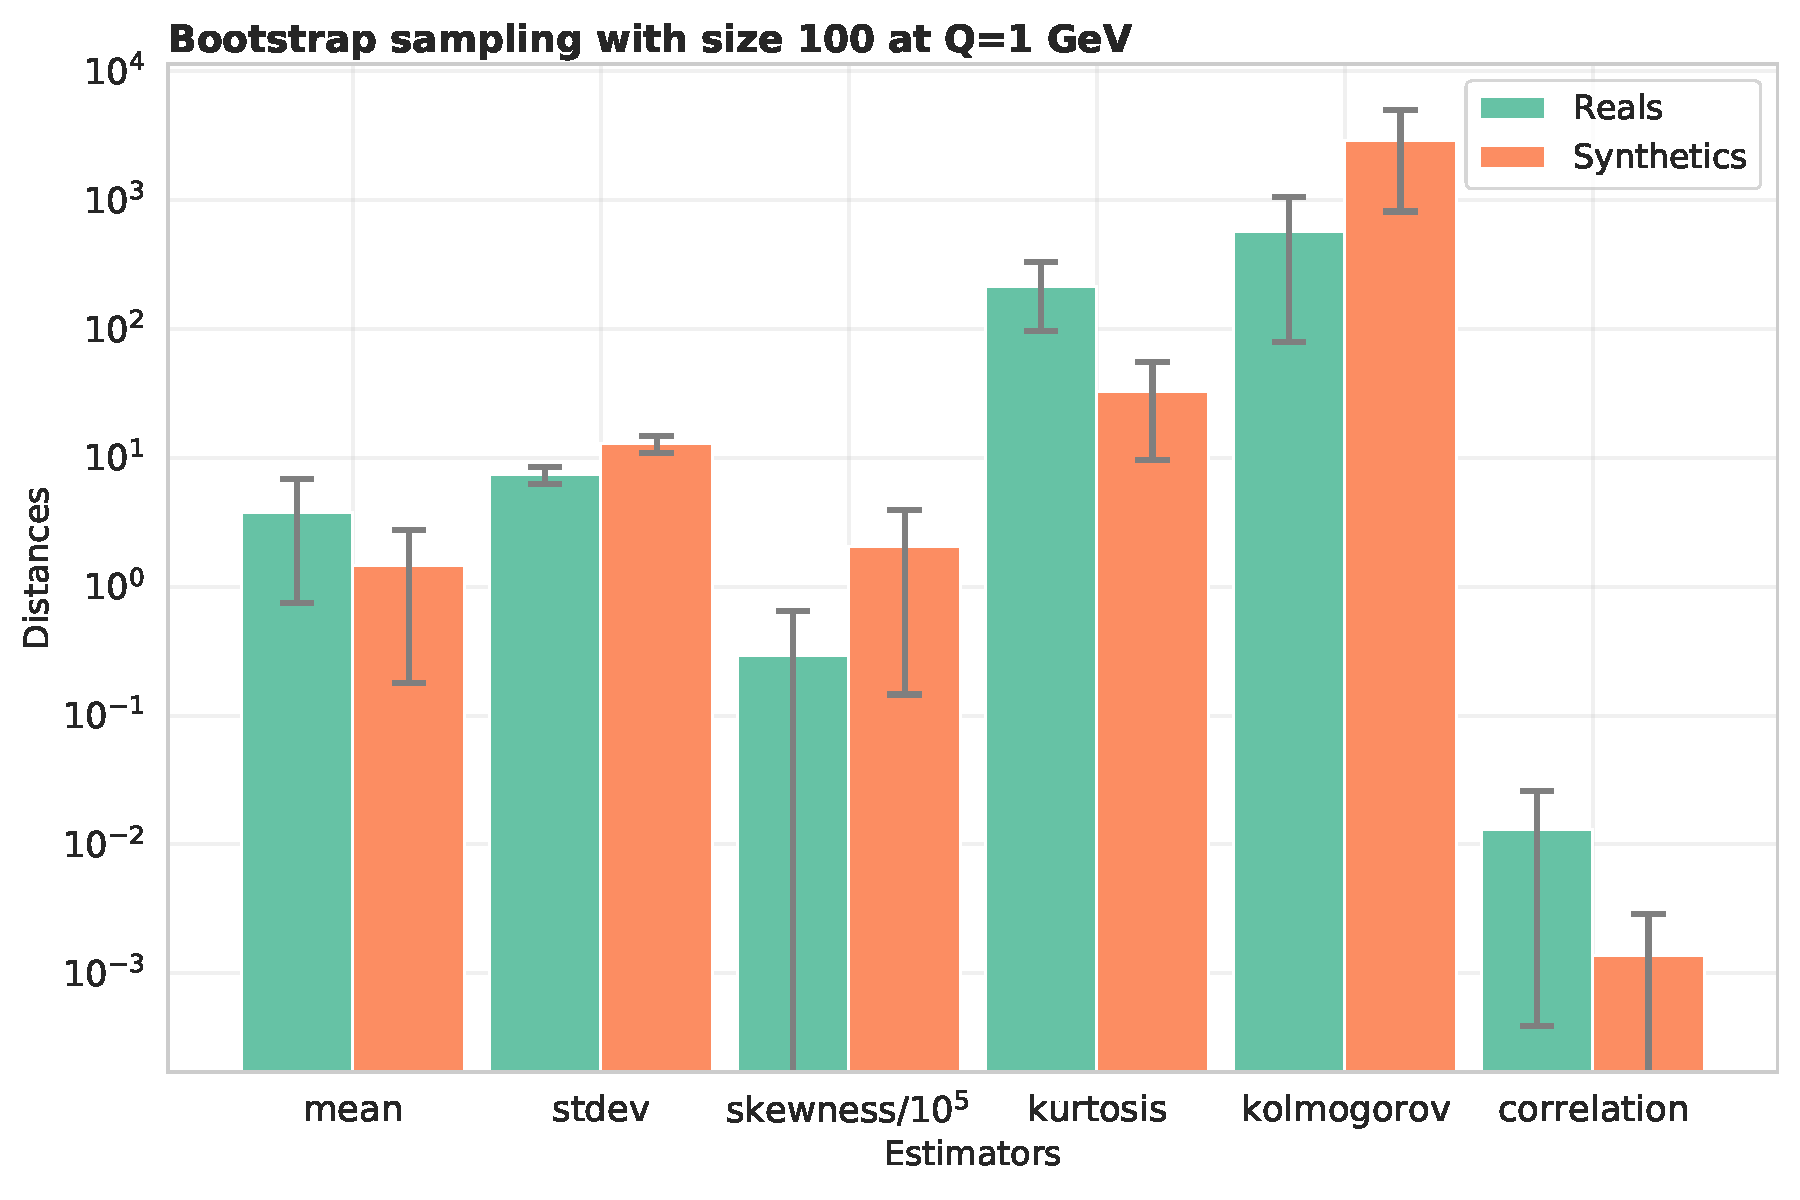
\includegraphics[width=\linewidth]{./gan_compressor/imgs/bootstrap.pdf}
		\end{column}
	\end{columns}
\end{frame}
